\documentclass[12pt]{article}
\usepackage[pdftex]{graphicx}
\newcommand{\kg}{\mathrm{kg}}
\newcommand{\m}{\mathrm{m}}
\newcommand{\cm}{\mathrm{cm}}
\newcommand{\s}{\mathrm{s}}
\newcommand{\ms}{\mathrm{ms}}
\newcommand{\N}{\mathrm{N}}
\newcommand{\vs}{\emph{vs}}
\newcounter{problem}
\stepcounter{problem}
\newcounter{answer}[problem]
\newenvironment{problem}{\noindent\begin{minipage}{\textwidth}\sloppy\sloppypar\raggedright\textbf{\theproblem.}\refstepcounter{problem}\stepcounter{answer}---}{\end{minipage}\vspace{2ex}}
\newcommand{\source}[1]{[{#1}]}
\newenvironment{answers}{\\}{}
\newcommand{\answer}[1]{\textbf{\Alph{answer}:}\refstepcounter{answer}~\mbox{#1}\hspace{3ex}}
\begin{document}

\section*{NYU General Physics 1---Term Exam 1}

\begin{problem}
  \source{from lecture 2011-09-06} Roughly what is the mass of a cube
  of rock of side length $10\,\m$?
  \begin{answers}
    \answer{$600\,\kg$}
    \answer{$60,000\,\kg$}
    \answer{$6,000,000\,\kg$}
    \answer{$600,000,000\,\kg$}
  \end{answers}
\end{problem}

\begin{problem}
  \source{from lecture 2011-09-08} How long does it take a heavy
  object to fall (from rest) about $5\,\m$?
  \begin{answers}
    \answer{much less than $0.01\,\s$}
    \answer{about $0.01\,\s$}
    \answer{about $0.1\,\s$}
    \answer{about $1\,\s$}
    \answer{much more than $1\,\s$}
  \end{answers}
\end{problem}

\begin{problem}
  \source{from lecture 2011-09-13} We spoke of a girl throwing a
  stone.  When the stone is precisely at the \emph{highest} point on
  its trajectory (at the apex), and ignoring air resistance, the
  acceleration of the stone:
  \begin{answers}
    \answer{is zero}
    \answer{is downwards at $9.8\,\m\,\s^{-2}$}
    \answer{depends on the velocity}
    \answer{is none of the above}
  \end{answers}
\end{problem}

\begin{problem}
  \source{from lecture 2011-09-15} Which of the following position
  \vs\ time graphs is a possible path for a car undergoing normal
  kinds of acceleration and deceleration?
  \\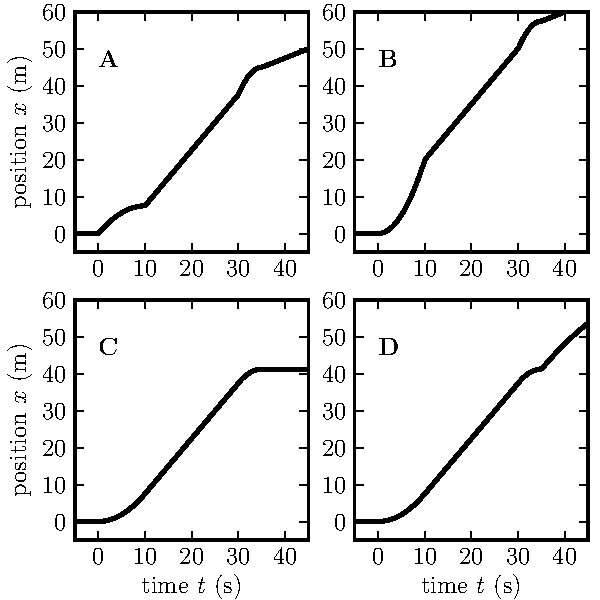
\includegraphics{../py/x_vs_t_options.pdf}
\end{problem}

\begin{problem}
  \source{from lecture 2011-09-20} What is the magnitude $|\vec{N}|$
  of the normal force for a block on a frictionless plane inclined at
  an angle $\theta$ to the horizontal?
  \begin{answers}
    \answer{$|\vec{N}| = m\,|\vec{g}|\,\cos\theta$}
    \answer{$|\vec{N}| = m\,|\vec{g}|\,\sin\theta$}
    \answer{$|\vec{N}| = |\vec{g}|\,\cos\theta$}
    \answer{$|\vec{N}| = |\vec{g}|\,\sin\theta$}
    \answer{$|\vec{N}| = m\,|\vec{g}|$}
  \end{answers}
\end{problem}

\begin{problem}
  \source{from lecture 2011-09-20} For the block on the inclined
  plane, by what method did we figure out the \emph{direction} of the
  acceleration?
  \begin{answers}
    \answer{Acceleration is always perpendicular to gravity.}
    \answer{Acceleration is always perpendicular to a normal force.}
    \answer{We used $\vec{F}=m\,\vec{a}$.}
    \answer{We used common sense and/or physical intuition.}
    \answer{We used none of the above.}
  \end{answers}
\end{problem}

\begin{problem}
  \source{from lecture 2011-09-22} We considered a machine that had
  two blocks, one $2\,\kg$, one $4\,\kg$, attached by a light string
  with tension $T_4$ in the string.  The $T_4$ string was draped over
  a light, fixed, frictionless pulley.  What is true of this tension
  $T_4$ (if we set $g=10\,\m\,\s^{-2}$)?
  \begin{answers}
    \answer{$T_4 = 20\,\N$}
    \answer{$20 < T_4 < 30\,\N$}
    \answer{$30 \leq T_4 < 40\,\N$}
    \answer{$T_4 = 40\,\N$}
    \answer{$T_4 > 40\,\N$}
  \end{answers}
\end{problem}

\begin{problem}
  \source{from lecture 2011-09-27} A plane is flying in a circular
  path at speed $v$.  The circle has radius $R$.  If the plane flies
  for a short time $t$, by what angle $\theta$ does its direction
  change during that time?
  \begin{answers}
    \answer{$\displaystyle\theta = \frac{R\,t}{v}$}
    \answer{$\displaystyle\theta = \frac{v}{R\,t}$}
    \answer{$\displaystyle\theta = \frac{R}{v\,t}$}
    \answer{$\displaystyle\theta = \frac{v\,t}{R}$}
    \answer{none of the above}
  \end{answers}
\end{problem}

\begin{problem}
  \source{from lecture 2011-09-29} A textbook of mass $m$ slams into a
  hard surface.  Before the collision, the textbook is moving at speed
  $v$.  The textbook stops in a time $\Delta t$.  After the collision,
  the textbook is at rest.  The magnitude of the force of impact is
  roughly
  \begin{answers}
    \answer{$\displaystyle m\,\frac{v}{\Delta t}$}
    \answer{$\displaystyle \frac{v}{\Delta t}$}
    \answer{$\displaystyle m\,\frac{\Delta t}{v}$}
    \answer{$\displaystyle \frac{\Delta t}{v}$}
  \end{answers}
\end{problem}

\begin{problem}
  \source{from problem set 1, problem 1} At 1500 dollars per ounce
  (29\,g), roughly what is the mass of $100$ million dollars worth of
  gold?
  \begin{answers}
    \answer{much less than $20\,\kg$}
    \answer{$20\,\kg$}
    \answer{$2,000\,\kg$}
    \answer{$200,000\,\kg$}
    \answer{much more than $200,000\,\kg$}
  \end{answers}
\end{problem}

\begin{problem}
  \source{from problem set 1, problem 2} What combination of length $L$,
  density $\rho$, and speed $v$ have dimensions of force?
  \begin{answers}
    \answer{$\rho\,L\,v$}
    \answer{$\rho\,L\,v^2$}
    \answer{$\rho\,L^2\,v$}
    \answer{$\rho\,L^2\,v^2$}
    \answer{none of the above}
  \end{answers}
\end{problem}

\begin{problem}
  \source{from problem set 1, problem 3} The dynamic viscosity $\mu$
  has dimensions of mass per length per time (units of
  $\kg\,\m^{-1}\,\s^{-1}$).  What combination of dynamic viscosity
  $\mu$, length $L$, and speed $v$ have units of force?
  \begin{answers}
    \answer{$\mu\,L\,v$}
    \answer{$\mu\,L\,v^2$}
    \answer{$\mu\,L^2\,v$}
    \answer{$\mu\,L^2\,v^2$}
    \answer{none of the above}
  \end{answers}
\end{problem}

\begin{problem}
  \source{from problem set 2, problem 1} A dragster travels 0.25\,mi
  in 5.5\,s, starting from rest.  Under the assumption of constant
  acceleration, what is the time it takes the dragster to go half-way;
  that is, how many seconds does it take to go the first 0.125\,mi?
  \begin{answers}
    \answer{substantially less than $1.38\,\s$}
    \answer{$1.38\,\s$}
    \answer{$2.75\,\s$}
    \answer{$3.9\,\s$}
    \answer{substantially more than $3.9\,\s$}
  \end{answers}
\end{problem}

\begin{problem}
  \source{from problem set 2, problem 1} Again, the dragster: Two cars
  start from rest and accelerate at constant acceleration over a
  distance $X$.  If car $F$ goes at twice the acceleration of car $S$,
  by what factor is car $S$ slower?  That is, what is the ratio of the
  time $t_S$ taken by car $S$ to the time taken by car $F$?
  \begin{answers}
    \answer{$1$}
    \answer{$\sqrt{2}$}
    \answer{$2$}
    \answer{$4$}
  \end{answers}
\end{problem}

\begin{problem}
  \source{from problem set 2, problem 2} Which of the following graphs
  is a possible graph of the velocity as a function of time for an
  object thrown upwards at $3\,\m\,\s^{-1}$ at $t=0$ and then falling
  freely?
  \\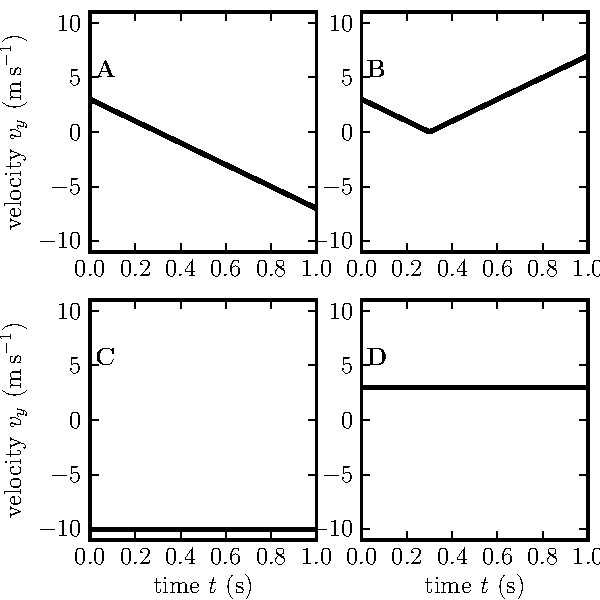
\includegraphics{../py/vy_vs_t_options.pdf}
\end{problem}

\begin{problem}
  \source{from problem set 2, problem 3} Below is a graph of velocity
  $v_x$ in the $x$ direction as a function of time for an automobile.
  \\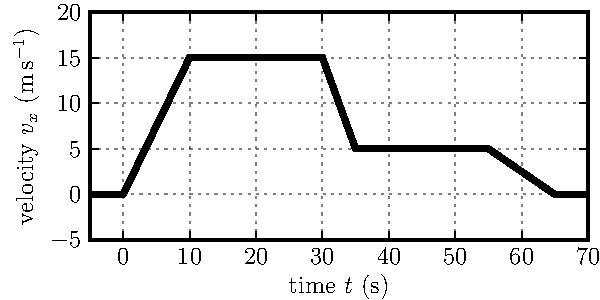
\includegraphics{../py/vx_vs_t.pdf}\\
  How far does the automobile travel between $t=0$ and $t=35\,\s$?
  \begin{answers}
    \answer{$5\,\m$}
    \answer{$175\,\m$}
    \answer{$425\,\m$}
    \answer{$525\,\m$}
    \answer{much more than $525\,\m$}
  \end{answers}
\end{problem}

\begin{problem}
  \source{from problem set 3, problem 1} If $g$ is the acceleration
  due to gravity and $R$ is the radius of the Earth, what, roughly, is
  the orbital period of the Space Station?
  \begin{answers}
    \answer{$\displaystyle 2\pi\,\sqrt{\frac{R}{g}}$}
    \answer{$\displaystyle 2\pi\,\sqrt{\frac{g}{R}}$}
    \answer{$\displaystyle 2\pi\,\sqrt{R\,g}$}
    \answer{$\displaystyle 2\pi\,\sqrt{\frac{1}{R\,g}}$}
    \answer{none of the above}
  \end{answers}
\end{problem}

\begin{problem}
  \source{from problem set 3, problem 2} What is the tension T in this
  problem?\\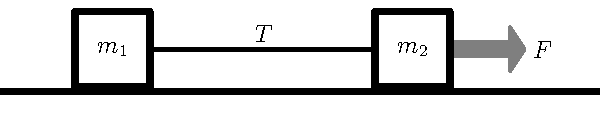
\includegraphics{../py/stringblocks.pdf}
  \begin{answers}
    \answer{$\displaystyle F\,\frac{m_1}{m_1+m_2}$}
    \answer{$\displaystyle F\,\frac{m_2}{m_1+m_2}$}
    \answer{$\displaystyle F$}
    \answer{$\displaystyle m_1\,g$}
    \answer{$\displaystyle m_2\,g$}
  \end{answers}
\end{problem}

\begin{problem}
  \source{from problem set 3, problem 3} A block of mass $m=9\,\kg$
  lies on a horizontal table.  It is stationary relative to the table.
  Now imagine that the table is accelerating upwards with an
  acceleration of magnitude $0.5\,\m\,\s^{-2}$.  What is the magnitude
  of the force on the block from the table?  For ease of calculation,
  take $g=10\,\m\,\s^{-2}$.
  \begin{answers}
    \answer{$4.5\,\N$}
    \answer{$85.5\,\N$}
    \answer{$90.0\,\N$}
    \answer{$94.5\,\N$}
    \answer{much more than $94.5\,\N$}
  \end{answers}
\end{problem}

\begin{problem}
  \source{from problem set 4, problem 1} A block of mass $m$ sits on a
  plane inclined at an angle of $\theta=20\,\deg$ to the horizontal.
  There is a coefficient of friction $\mu=0.9$ between the block and
  the plane.  What is the magnitude of the frictional force?
  \begin{answers}
    \answer{$m\,g\,\cos\theta$}
    \answer{$m\,g\,\sin\theta$}
    \answer{$\mu\,m\,g\,\cos\theta$}
    \answer{$\mu\,m\,g\,\sin\theta$}
    \answer{$\mu\,m\,g\,\tan\theta$}
  \end{answers}
\end{problem}

\begin{problem}
  \source{from problem set 4, problem 2} At the lowest point in its
  swing, a mass swinging like a pendulum at the end of a light,
  inextensible string is
  \begin{answers}
    \answer{not accelerating}
    \answer{accelerating upwards}
    \answer{accelerating downwards}
    \answer{accelerating in the direction of the velocity}
    \answer{accelerating in the direction opposite to the velocity}
  \end{answers}
\end{problem}

\begin{problem}
  \source{from problem set 4, problem 3} A ball of mass $m$ and radius
  $R$ drops from a height $h$ onto a flat surface.  It bounces.  In
  which of these situations will the contact force (during the bounce)
  be largest?
  \begin{answers}
    \answer{rubber ball on rubber surface}
    \answer{rubber ball on marble surface}
    \answer{steel ball on rubber surface}
    \answer{steel ball on marble surface}
  \end{answers}
\end{problem}

\begin{problem}
  \source{from \textit{Motion 1} lab} The motion sensor measured the
  position of your notebook by making use of
  \begin{answers}
    \answer{the volume of reflected sound pulses}
    \answer{the brightness of reflected light pulses}
    \answer{the arrival times of reflected sound pulses}
    \answer{the arrival times of reflected light pulses}
    \answer{none of the above}
  \end{answers}
\end{problem}

\begin{problem}
  \source{from \textit{Motion 2} lab} Take the second derivative with respect
  to time $t$ of the expression $$x_0 + v_0\,t +
  \frac{1}{2}\,a\,t^2$$.  What do you get?
  \begin{answers}
    \answer{$\displaystyle x_0 + v_0\,t + \frac{1}{2}\,a\,t^2$}
    \answer{$\displaystyle x_0 + v_0\,t$}
    \answer{$\displaystyle x_0$}
    \answer{$\displaystyle v_0 + a\,t$}
    \answer{$\displaystyle a$}
  \end{answers}
\end{problem}

\begin{problem}
  WRONG ANSWERS \source{from \textit{Equilibrium of a Particle} lab} Imagine that
  there are three forces $\vec{A}$, $\vec{B}$ and $\vec{C}$ acting on
  a particle such that the particle is in equilibrium.  Now imagine
  that forces $\vec{B}$ and $\vec{C}$ point in opposite directions from one another.
  What is true of the force magnitudes?
  \begin{answers}
    \answer{$|\vec{A}|^2 = |\vec{B}|^2 + |\vec{C}|^2$}
    \answer{$|\vec{A}|^2 = |\vec{B}|^2 + |\vec{C}|^2 - |\vec{B}|\,|\vec{C}|\,\cos{\theta}$}
    \answer{$|\vec{A}| = 0$ and $|\vec{B}| = |\vec{C}|$}
    \answer{All forces must have zero magnitude.}
    \answer{None of the above.}
  \end{answers}
\end{problem}

\end{document}
